\documentclass[convert={outext=.png}]{standalone}
\usepackage{tikz}

\thispagestyle{empty}

\begin{document}
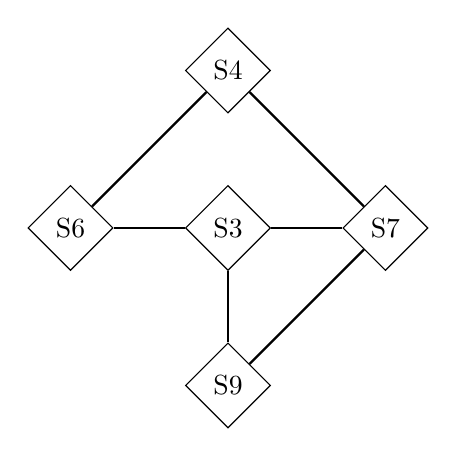
\begin{tikzpicture}
  \usetikzlibrary{positioning,matrix,arrows,shapes}



       \tikzstyle{arrow} = [thick,->,>=stealth]
       \tikzset{switch/.style = {diamond, draw, text centered, minimum height=2e
m, node distance= 2cm}, }
       \tikzset{router/.style = {rectangle, draw, text centered, minimum height=
2em}, }
       \tikzset{host/.style = {circle, draw, text centered, minimum height=2em},
 }
       \tikzset{ftable/.style={rectangle, dashed, draw} }
       \node[switch] (S3) {S3};
       \node[switch, left of=S3] (S6) {S6};
       \node[switch, right of=S3] (S7) {S7};
       \node[switch, above of=S3] (S4) {S4};
       \node[switch, below of=S3] (S9) {S9};
 
       \path[draw,thick]
       (S3) edge (S6) 
       (S3) edge (S7) 
       (S6) edge (S4) 
       (S4) edge (S7)
       (S3) edge (S9)
       (S9) edge (S7)
       (S3) edge (S7); 


\end{tikzpicture}
\end{document}
